
To understand the specific characteristics of PaaS-hosted web APIs, and the potential
of this restricted domain to facilitate efficient static analysis and response time 
prediction,  we next summarize results from static analysis (using the Soot
framework~\cite{Vallee-Rai:2010:SJB:1925805.1925818}) of 
35 real world App Engine web APIs. These web APIs are open 
source, written in Java, and run over Google App Engine or AppScale without modification.
We plan to make these applications publicly available upon publication.  
%We omit data graphs due to space constraints.

\begin{figure}
\centering
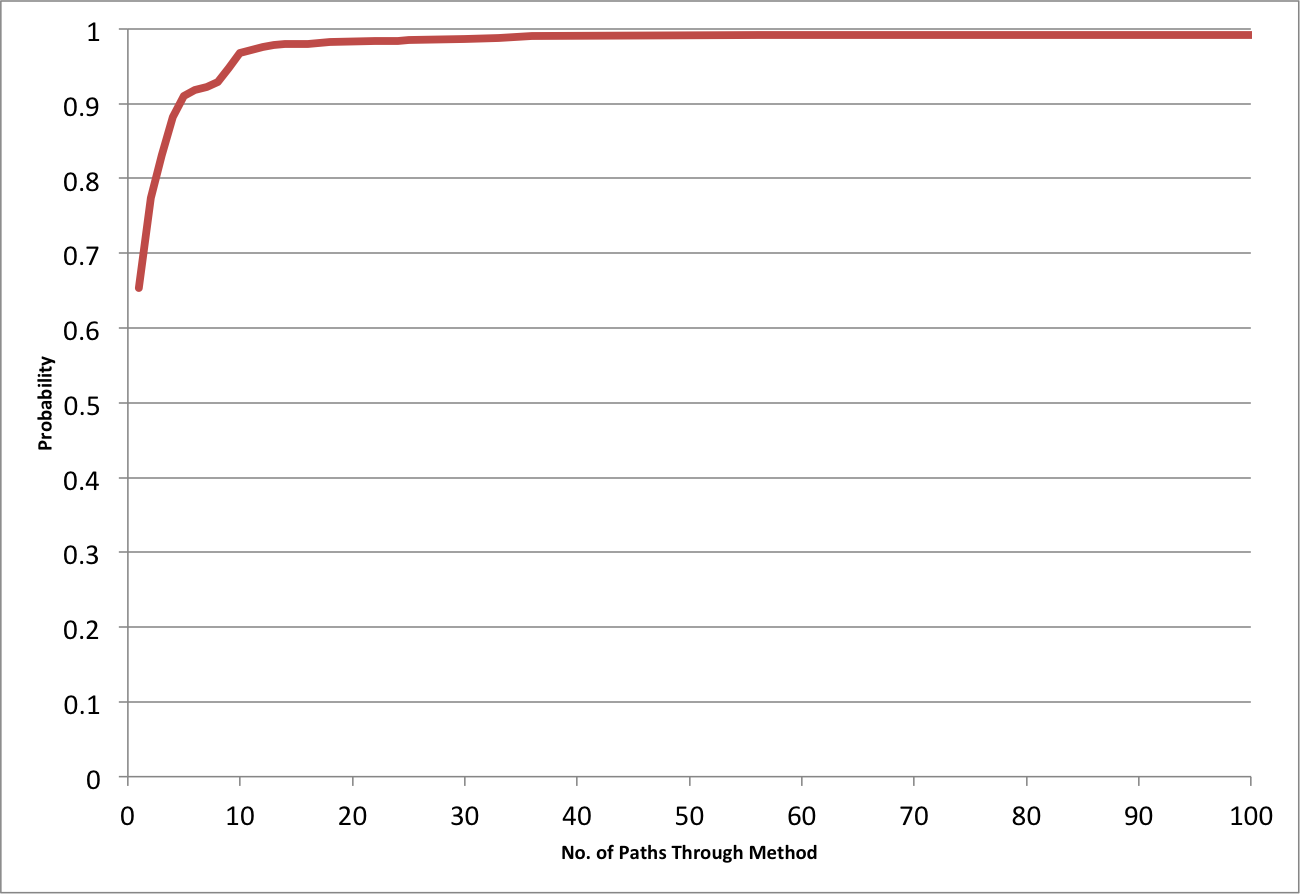
\includegraphics[scale=0.35]{path_count_cdf}
\caption{CDF of the number of static paths through methods in the surveyed web APIs.
\label{fig:path_count_cdf}
}
\vspace{-0.2in}
\end{figure}

Our analysis detected a total of 1458 Java methods in the analyzed codes.
Figure~\ref{fig:path_count_cdf} shows the cumulative distribution of 
static program paths in these methods.
Approximately 97\% of the methods considered in the analysis have 10 or fewer 
static program paths through them.  99\% of 
the methods have 36 or fewer paths.
However, the CDF is heavy tailed, and grows to 34992.
We truncate the graph at 100 paths for clarity. As such, 
only a very small number of methods 
each contains a large number of paths.
Fortunately, over 65\% of the methods have exactly 1 path (i.e. there are no branches).

Next, we consider the looping behavior of web APIs.  1286 of the methods (88\%)
considered in the study
do not have any loops. 172 methods (12\%) contain loops. 
We believe that this characteristic is due to the fact that 
the PaaS SDK and the platform restrictions like quotas and response time limits 
discourage looping.

Approximately 29\% of all the loops in 
the analyzed programs do not contain any cloud SDK invocations. 
A majority of the loops (61\%) however, are
used to iterate over a dataset that is returned from the datastore cloud SDK interface 
of App Engine (i.e iterating on the result set 
returned by a datastore query). We refer to this particular type of 
loops as \textit{iterative datastore reads}. 
%We use these heuristics when designing the loop handling capability of Cerebro.

%\begin{table}[htdp]
\begin{table}
\caption{Static cloud SDK calls in surveyed web APIs
\label{tab:sdk_call_counts}
}
\begin{center}
\begin{tabular}{|c|c|}
\hline
Cloud SDK Interface & No. of Invocations \\ \hline
blobstore & 7 \\ \hline
channel & 1 \\ \hline
datastore & 735 \\ \hline
files & 4 \\ \hline
images & 3 \\ \hline
memcache & 12 \\ \hline
search & 6 \\ \hline
taskqueue & 24 \\ \hline
tools & 2 \\ \hline
urlfetch & 8 \\ \hline
users & 44 \\ \hline
xmpp & 3 \\ \hline
\end{tabular}
\end{center}
\vspace{-0.2in}
\end{table}

Table~\ref{tab:sdk_call_counts} lists the number of times each cloud 
SDK interface is called across all paths and methods in the analyzed programs.
The Datastore API is the most commonly used interface.
This is because data management is fundamental 
to most web APIs and the PaaS
disallows using the local filesystem to do so,
for scalability and portability reasons.

\begin{figure}
\centering
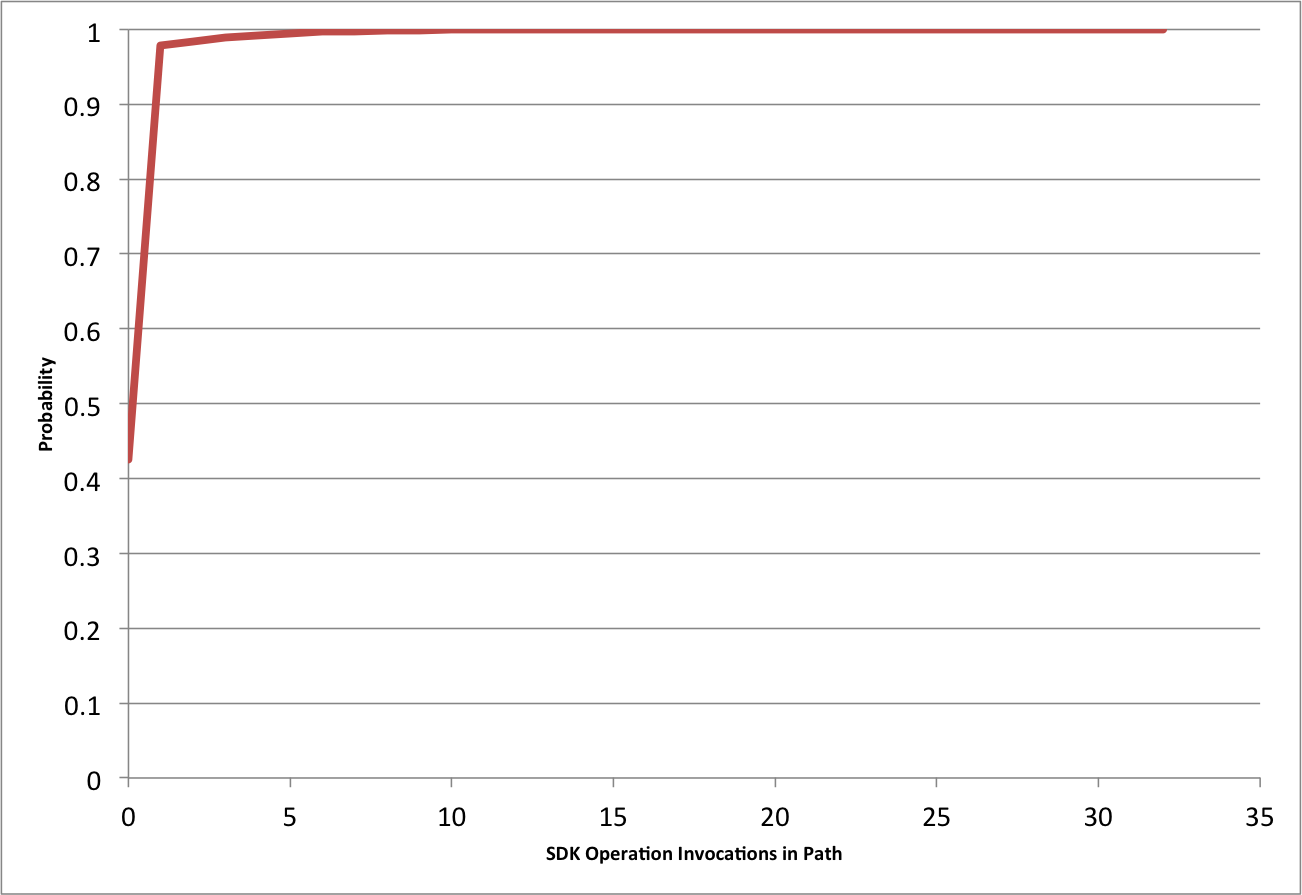
\includegraphics[scale=0.35]{sdk_call_count_cdf}
\caption{CDF of cloud SDK call counts in paths of execution.
\label{fig:sdk_call_count_cdf}
}
\vspace{-0.1in}
\end{figure}

Next, we explore the number of cloud SDK calls made along 
different paths of execution in the web APIs. For this study
we consider all paths of execution through the methods (64780 total paths). 
Figure~\ref{fig:sdk_call_count_cdf}
shows the cumulative distribution of the number of SDK calls within paths.
Approximately 98\% of the paths have 1 cloud SDK call or fewer. 
The probability of finding an execution path with more than
5 cloud SDK calls is smaller than 1\%.
%This implies in most cases Cerebro will likely be able to make response 
%time predictions by analyzing the
%historical performance data of a very small number of cloud SDK operations.

Finally, our experience with App Engine web APIs indicates that a significant
portion of the total time of a method (web API operation) is spent in cloud SDK calls.
Confirming this hypothesis requires careful instrumentation (i.e. difficult
to automate) of the web API codes.  We performed such a test by hand on two 
representative applications and found that the time spent in code other than cloud SDK calls
accounts for $0$-$6$\% of the total time (0-3ms for a 30-50ms web API operation).

This study of various characteristics typical of 
PaaS-hosted web APIs indicates that there may be 
opportunities to exploit the specific aspects of this
application domain to simplify analysis and to facilitate
performance prediction.  In particular, operations in these applications
are short, have a small number of paths to analyze, implement few
loops, and invoke a small number of cloud SDK calls. Moreover, most
of the time spent executing these operations results from cloud SDK invocations.
In the next section, we describe our design and implementation of Cerebro
that takes advantage of these characteristics and assumptions.
We then use a Cerebro prototype to experimentally evaluate its efficacy
for estimating the worst-case response time for 
applications from this domain.
